\documentclass{article}

\usepackage{graphicx}
\usepackage{rotating}
\usepackage{amsmath}
\usepackage{amssymb}
\usepackage{fancyhdr}
\usepackage{listings}
%\usepackage{xcolor}
\usepackage{color}
\usepackage{amsfonts}
\usepackage{textcomp}
\usepackage{float}
\usepackage{longtable}
\usepackage[sorting=none]{biblatex}
\usepackage[margin=1in]{geometry}
\usepackage[font={small,it}]{caption}
\usepackage[table,xcdraw]{xcolor}
\usepackage{placeins}
\usepackage{xepersian}





%\DeclareMathOperator*{\btie}{\bowtie}
\addbibresource{bibliography.bib}
\settextfont[Scale=1.2]{B-NAZANIN.TTF}
\setlatintextfont[Scale=1]{Times New Roman}
\renewcommand{\baselinestretch}{1.5}
\pagestyle{fancy}
\fancyhf{}
\rhead{تکلیف تئوری دوم درس کامپایلر}
\lhead{\thepage}
\rfoot{علیرضا ابره فروش}
\lfoot{9816603}
\renewcommand{\headrulewidth}{1pt}
\renewcommand{\footrulewidth}{1pt}
%%%%%%%%%%
\lstset
{
    language=[latex]tex,
    basicstyle=\ttfamily,
    commentstyle=\color{black},
    columns=fullflexible,
    keepspaces=true,
    upquote=true,
    showstringspaces=false,
    morestring=[s]\\\%,
    stringstyle=\color{black},
}
%%%%%%%%%%
%beginMatlab
\definecolor{mygreen}{RGB}{28,172,0} % color values Red, Green, Blue
\definecolor{mylilas}{RGB}{170,55,241}
%endMatlab
\begin{document}
%beginMatlab
\lstset{language=Matlab,%
    %basicstyle=\color{red},
    breaklines=true,%
    morekeywords={matlab2tikz},
    keywordstyle=\color{blue},%
    morekeywords=[2]{1}, keywordstyle=[2]{\color{black}},
    identifierstyle=\color{black},%
    stringstyle=\color{mylilas},
    commentstyle=\color{mygreen},%
    showstringspaces=false,%without this there will be a symbol in the places where there is a space
    numbers=left,%
    numberstyle={\tiny \color{black}},% size of the numbers
    numbersep=9pt, % this defines how far the numbers are from the text
    emph=[1]{for,end,break},emphstyle=[1]\color{red}, %some words to emphasise
    %emph=[2]{word1,word2}, emphstyle=[2]{style},    
}
%endMatlab
\begin{titlepage}
\begin{center}

\includegraphics[width=0.4\textwidth]{figures/IUT Logo.png}\\
        
\LARGE
\textbf{دانشگاه صنعتی اصفهان}\\
\textbf{دانشکده مهندسی برق و کامپیوتر}\\
        
\vfill
        
\huge
\textbf{عنوان: تکلیف چهارم درس ریزپردازنده}\\
        
\vfill
        
\LARGE
\textbf{نام و نام خانوادگی: علیرضا ابره فروش}\\
\textbf{شماره دانشجویی: 9816603}\\
\textbf{نیم\,سال تحصیلی: پاییز 1400}\\
\textbf{مدرّس: دکتر عارف کریمی افشار}\\
\end{center}
\end{titlepage}


%\tableofcontents
\newpage

\section{}%1
\subsection{\lr{a}}
طبق الگوریتم زیر عمل می‌کنیم.
\begin{figure}[H]
    \centering
    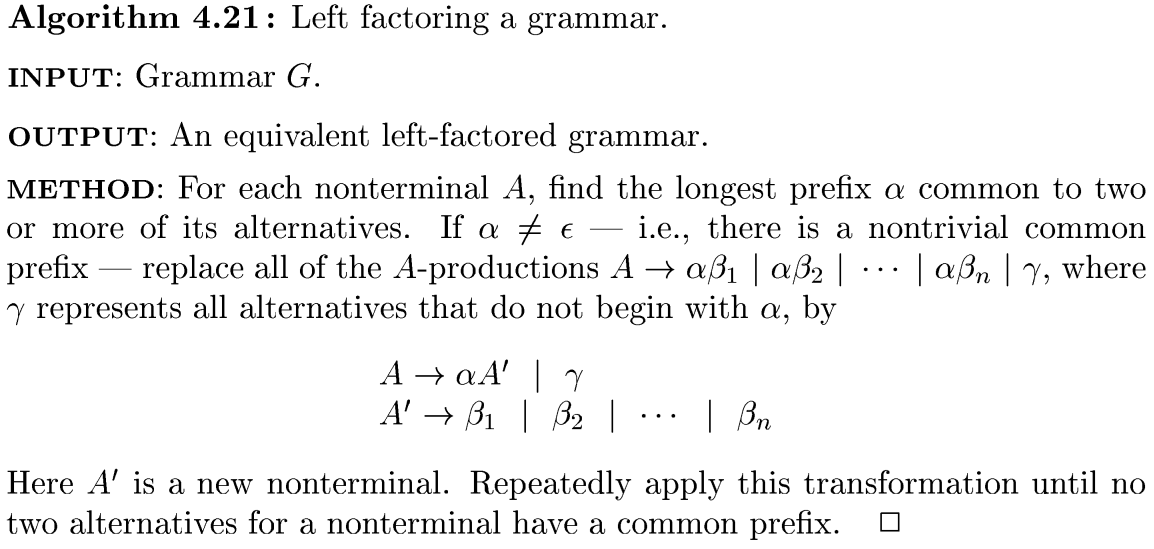
\includegraphics[width=0.75\textwidth]{figures/1a.png}
    \caption
	{}
    \label{fig:fig1}
\end{figure}

\begin{latin}
$
S \longrightarrow SS ^ \prime \\
S ^ {\prime} \longrightarrow +S|+P \\
P \longrightarrow PP ^ \prime \\
P ^ \prime \longrightarrow *P|*I \\
I \longrightarrow -I|(S)|D \\
D \longrightarrow 0|1N \\
N \longrightarrow NN ^ \prime|0|1|\varepsilon \\
N ^ \prime \longrightarrow N
$
\end{latin}

\subsection{\lr{b}}
طبق الگوریتم زیر عمل می‌کنیم.
\begin{figure}[H]
    \centering
    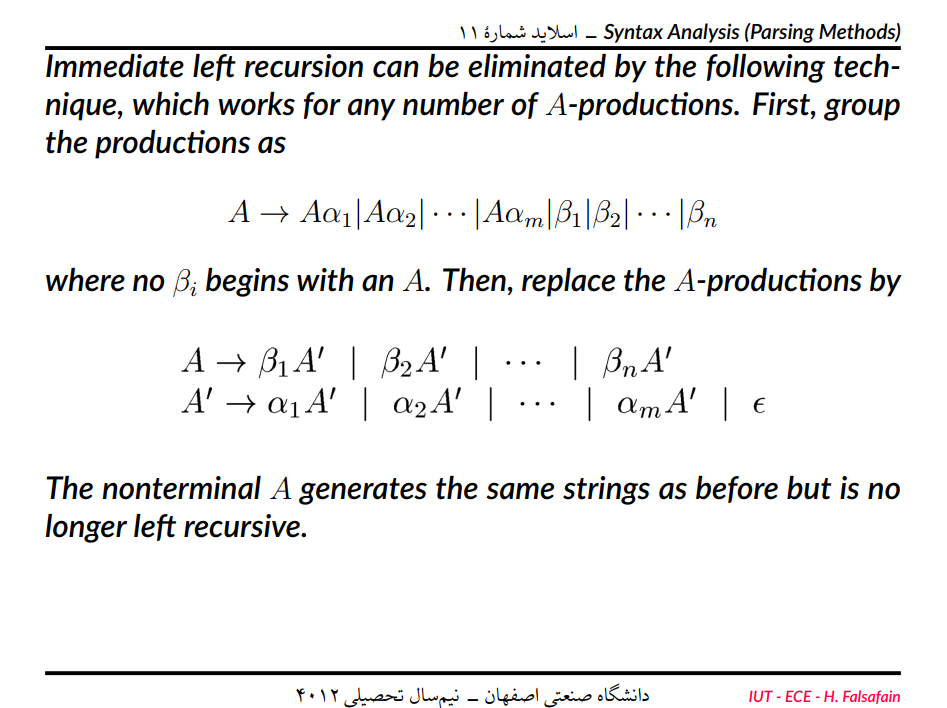
\includegraphics[width=0.75\textwidth]{figures/1b.png}
    \caption
	{}
    \label{fig:fig1}
\end{figure}

\begin{latin}
$
S \longrightarrow US ^ \prime \\
S ^ \prime \longrightarrow aSS ^ \prime | \varepsilon \\
U \longrightarrow TU ^ \prime \\
U ^ \prime \longrightarrow uUU ^ \prime | \varepsilon \\
T \longrightarrow tT ^ \prime | fT ^ \prime | (S)T ^ \prime \\
T ^ \prime \longrightarrow | nT ^ \prime | \varepsilon
$
\end{latin}
















\section{}%1
\subsection{}
خطاهای شناسایی شده توسط تحلیلگر لغوی معمولا دارای ویژگی های زیر هستند:
\begin{itemize}
\item این خطاها زمانی رخ می‌دهند که دنباله ورودی از کاراکترهای معتبر در زبان برنامه‌نویسی مورد نظر تشخیص داده نمی‌شود.
\item این خطاها به طور کلی توسط تحلیلگر لغوی تشخیص داده می‌شوند که در مرحله اول فرایند کامپایل است.
\item این خطاها اغلب به دلیل خطاهای نحوی، مانند کلمات کلیدی یا شناسه‌های نوشتاری نادرست یا کاراکترهای نامعتبر یا نمادها ایجاد می‌شوند.
\end{itemize}

\subsection{}
چهار نمونه مختلف از انواع خطاهای شناسایی شده توسط تحلیل‌گر لغوی، شامل موارد زیر می‌شوند:

\begin{enumerate}
\item کاراکترهای غیرمجاز: این کاراکترها که در زبان برنامه‌نویسی شناخته نشده‌اند، مانند کاراکترهای غیر چاپ‌پذیر یا نویسه‌هایی از زبان‌های دیگر هستند.
\item عدم تطابق نقل قول: این خطا هنگامی رخ می‌دهد که یک متن رشته‌ای به درستی با نقل قول متناظر خاتمه نمی‌یابد. به عنوان مثال، \lr{"Hello، World!} احتمالاً به دلیل عدم وجود دابل کوتیشن پایانی، با خطای لغوی روبرو می‌شود.
\item
\end{enumerate}

\section{}%2

کامپایلر برنامه‌ای است که می تواند یک برنامه از یک زبان (زبان منبع) را بخواند و آن را به یک برنامه معادل به زبان دیگری (زبان هدف) ترجمه کند. نقش مهمی که کامپایلر ایفا می‌کند، گزارش هر نوع خطایی در برنامه‌ی منبع است که در طول فرآیند ترجمه تشخیص داده می‌شود.











%%%%%%%%%%%%%%%%%%%%%%%%%%%%%%%%%%%%%%%%%%%%%%%%%%%%%%%%%%%%%%%%%%%%%%

%\begin{latin}
%\lstinputlisting{sources/p2.m}
%\end{latin}


%%%%%%%%%%%%%%%%%%%%%%%%%%%%%%%%%%%
%%%%%%%%%%%%%%%%%%%%%%%%%%%%%%%%%%%
%%%%%%%%%%%%%%%%%%%%%%%%%%%%%%%%%%%

%------------------------------------------------------------------------------------------


\subsection*{منابع}
\renewcommand{\subsection}[2]{}%
\begin{thebibliography}{99} % assumes less than 100 references
%چنانچه مرجع فارسی نیز داشته باشید باید دستور فوق را فعال کنید و مراجع فارسی خود را بعد از این دستور وارد کنید


\begin{LTRitems}

\resetlatinfont

\bibitem{b1}
\end{LTRitems}

\end{thebibliography}


\end{document}
